\documentclass[letter,11pt]{article}

\usepackage[spanish,es-nodecimaldot]{babel}
\usepackage[utf8]{inputenc}

\usepackage{lmodern}
\usepackage[T1]{fontenc}
\usepackage{textcomp}

\usepackage{framed}
\usepackage[svgnames]{xcolor}
\colorlet{shadecolor}{Gainsboro!50}

\usepackage[labelfont=bf]{caption}
\usepackage{graphicx}
\usepackage{pstricks}

\usepackage{anysize}
\marginsize{3cm}{2cm}{2cm}{3cm}

\usepackage{url}
\usepackage{siunitx}
\usepackage{amsmath}
\usepackage{array}
\usepackage{alltt}

\usepackage{caption}
\newcommand{\source}[1]{\vspace{-11pt} \caption*{\small{\textbf{Nota:} {#1}}}}

\usepackage{fancyhdr}
\usepackage{lastpage}
\pagestyle{fancy}
\fancyhf{}
\fancyhead[LE,RO]{Laboratorio de Física Básica II}
\fancyfoot[CO,CE]{\thepage\ de \pageref{LastPage}}

\special{papersize=215.9mm,279.4mm}

\usepackage[
    pdfauthor={Carlos Eduardo Caballero Burgoa},%
    pdftitle={Laboratorio de Física Básica II},%
    pdfsubject={Péndulo simple},%
    colorlinks,%
    citecolor=black,%
    filecolor=black,%
    linkcolor=black,%
    urlcolor=black,
    breaklinks]{hyperref}
\usepackage{breakurl}

\newcommand{\blankpage}{
\newpage
\thispagestyle{empty}
\mbox{}
\newpage
}

\renewcommand{\arraystretch}{1.2}

\title{Informe 3: Péndulo simple}
\author{Carlos Eduardo Caballero Burgoa \\
    \small{\href{mailto:200201226@est.umss.edu}{200201226@est.umss.edu}}
}
\date{28 de abril de 2021}

\begin{document}

\maketitle
\begin{center}
    \textbf{Grupo}: J2 (Miércoles)\\
    \textbf{Docente}: Ing. Milka Mónica Torrico Troche\\
    \textbf{Carrera}: Ing. Electromecánica
\end{center}

\begin{abstract}
Este documento detalla el experimento realizado en simulador para hallar la
relación funcional entre el periodo de oscilación ($T$) y la longitud ($L$) de
un péndulo simple, además de calcular el valor de la aceleración de la gravedad;
para esto se realizó dos mediciones de 10 oscilaciones de un péndulo con una
longitud determinada; y posteriormente se calcula la relación funcional después
de linealizar la curva y ajustarla con el método de mínimos cuadrados,
finalmente se determinó el valor de la gravedad, resultando ser igual a:
$(9.85 \pm 0.03)[m/s^2]; 0.33\%$.
\end{abstract}

\section{Introducción}

Un péndulo simple es un modelo idealizado que consiste en una masa puntual
suspendida de una cuerda no expansible y de masa despreciable. Si la masa se
mueve a un lado de su posición de equilibrio vertical descendente, oscilará
alrededor de dicha posición \cite{Young&Freedman}.

\begin{figure}
\centering
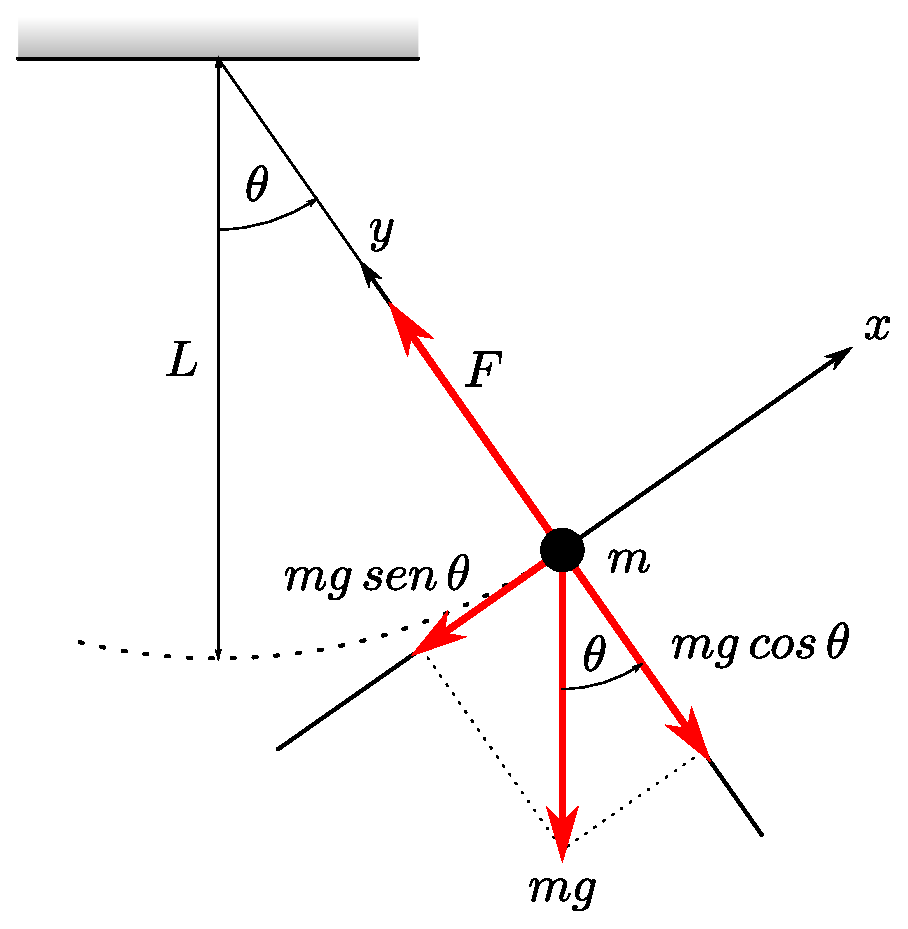
\includegraphics[width=0.38\textwidth]{resources/f1.eps}
\caption{Péndulo simple idealizado.}
\label{figura1}
\source{Física Universitaria Volumen I (p. 454), \\
Young, Hugh D. y Freedman, Roger A., 2013, Pearson.}
\end{figure}

En la \textbf{Figura \ref{figura1}} se detallan las fuerzas que actúan sobre la
masa ($m$) en cualquier instante del movimiento, estas fuerzas son: La tensión
($F$) de la cuerda y la fuerza de gravedad ($mg$), que se descompone en función
del ángulo desplazado ($\theta$), en una componente normal ($mg\, cos\, \theta$)
y una componente tangencial ($mg\, sen\, \theta$) \cite{GUIA}.

Aplicando la segunda ley de \emph{Newton} en la dirección tangencial, se
obtiene:

\begin{equation*}
    -mg\, sen\, (\theta) = m\, a_t
\label{segundaley}
\end{equation*}
\vspace{0.10cm}

La aceleración en la dirección tangencial es:

\begin{equation*}
    a_t = \frac{d^2 S}{dt^2}
\end{equation*}
\vspace{0.10cm}

Donde $S$ es la longitud del arco o trayectoria circular, cuya relación con el
ángulo $\theta$ y la longitud de la cuerda $L$ es:

\begin{equation*}
    S = \theta\, L
\end{equation*}
\vspace{0.10cm}

Por tanto:

\begin{equation*}
    \frac{d^2 \theta}{dt^2} + \frac{g}{L} sen\, (\theta) = 0
\end{equation*}
\vspace{0.10cm}

Si se consideran tan solo oscilaciones de pequeña amplitud, de modo que el
ángulo $\theta$ sea siempre suficientemente pequeño, entonces el valor del
$sen\, (\theta)$ será muy próximo al valor de $\theta$ expresado en radianes
($sen\, (\theta) \cong \theta$, para $\theta$ suficientemente pequeño), como
se aprecia en el \textbf{Cuadro \ref{cuadro1}} \cite{WIKI1}.

\begin{table}[!h]
\begin{center}
\begin{tabular}{|>{\centering}m{0.50cm}<{\centering}
                |>{\centering}m{1.25cm}<{\centering}
                |>{\centering}m{1.25cm}<{\centering}
                |>{\centering}m{2.50cm}<{\centering}|
                |>{\centering}m{0.50cm}<{\centering}
                |>{\centering}m{1.25cm}<{\centering}
                |>{\centering}m{1.25cm}<{\centering}
                |>{\centering}m{2.50cm}<{\centering}|}
\hline
$\theta [^\circ]$ & $\theta [rad]$ & $sen\, (\theta)$ & diferencia (\%) &
$\theta [^\circ]$ & $\theta [rad]$ & $sen\, (\theta)$ & diferencia (\%)
    \tabularnewline \hline
\hline
 0 & 0.00000 & 0.00000 & 0.00 & 15 & 0.26180 & 0.25882 & 1.15
    \tabularnewline \hline
 2 & 0.03491 & 0.03490 & 0.02 & 20 & 0.34907 & 0.34202 & 2.06
    \tabularnewline \hline
 5 & 0.08727 & 0.08716 & 0.13 & 25 & 0.43633 & 0.42262 & 3.25
    \tabularnewline \hline
10 & 0.17453 & 0.17365 & 0.51 & 30 & 0.52360 & 0.50000 & 4.72
    \tabularnewline \hline
\end{tabular}
\caption{Comparación entre el valor del ángulo y su función seno.}
\label{cuadro1}
\source{Adaptado de péndulo simple (Wikipedia).}
\end{center}
\end{table}

La ecuación anterior se reduce a:

\begin{equation*}
    \frac{d^2 \theta}{dt^2} + \frac{g}{L} \theta = 0
\label{oscilador}
\end{equation*}
\vspace{0.10cm}

La \textbf{Ecuación \ref{oscilador}} corresponde a un \textbf{oscilador armónico
simple} cuya solución general es:

\begin{equation*}
    \theta(t) = A\, cos\, (\omega\, t + \phi)
\end{equation*}
\vspace{0.10cm}

Donde $A$ representa el máximo desplazamiento angular de $\theta$, $\omega$ es
la frecuencia angular, y $\phi$ el desfase. Tanto la magnitud $A$, como $\phi$
son dos constantes determinadas por las condiciones iniciales.

La frecuencia angular ($\omega$) esta determinada por:

\begin{equation*}
    \omega = \sqrt{\frac{g}{L}}
\end{equation*}
\vspace{0.10cm}

Considerando que $\omega = 2\pi / T$, el periodo de oscilación para el péndulo
simple es:

\begin{equation}
    T = 2\pi\, \sqrt{\frac{L}{g}} = \frac{2\pi}{\sqrt{g}} \sqrt{L}
\label{periodo}
\end{equation}
\vspace{0.10cm}

Para el experimento se verificará la \textbf{Ecuación \ref{periodo}}.
A partir de una longitud de cuerda establecida ($L$), se medirá el tiempo de
oscilación del péndulo para hallar el periodo ($T$). Finalmente se determinará
el valor de la gravedad ($g$) despejándola de la misma ecuación.

\section{Método experimental}

\begin{figure}
\centering
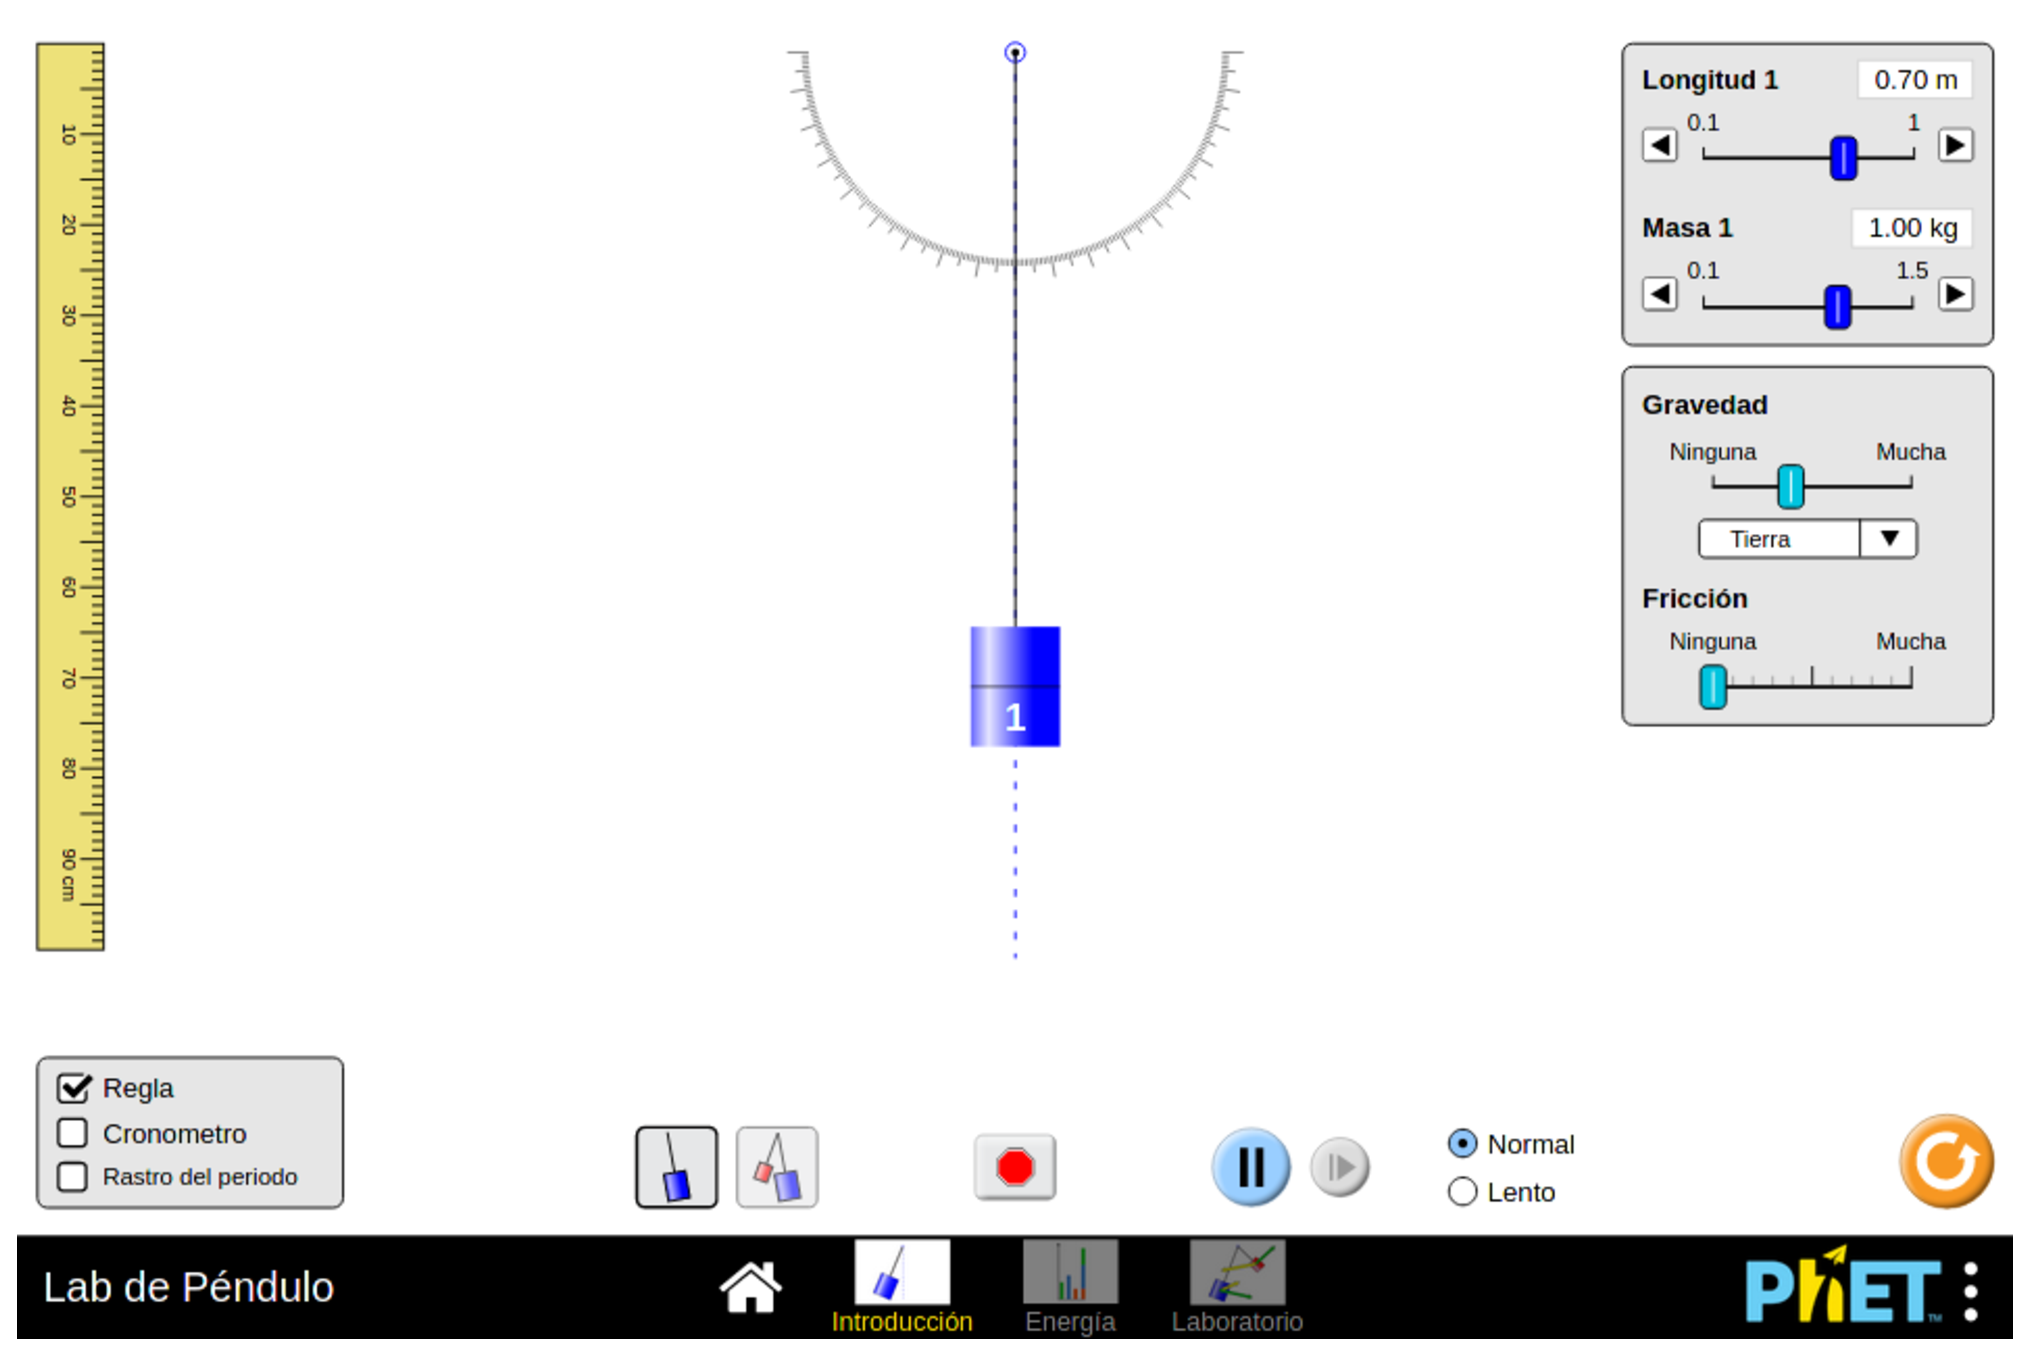
\includegraphics[width=0.90\textwidth]{resources/f2.eps}
\caption{Simulador de péndulo simple.}
\label{figura2}
\source{Captura propia.}
\end{figure}

Para la realización del experimento, se emplea el simulador de péndulo simple de
\emph{PHET}, ubicado en la dirección web: \url{
https://phet.colorado.edu/sims/html/pendulum-lab/latest/pendulum-lab_es.html},
tal como presenta en la \textbf{Figura \ref{figura2}}.

Para el simulador se escoge un valor de longitud ($L$), que se mantendrá
constante durante la medición, y se registrarán 2 veces la cantidad de tiempo
que requiere el péndulo para hacer 10 oscilaciones completas. Todas las
mediciones con una inclinación de $8^\circ$.

Una vez medidos los datos para 10 valores distintos de longitud ($L$), se
procederá a calcular el periodo ($T$) con la siguiente ecuación:

\begin{equation}
    T = \frac{\bar{t}}{10}
\label{periodo10}
\end{equation}
\vspace{0.10cm}

Donde $\bar{t}$, es el promedio de las mediciones realizadas.

Luego se procederá a graficar la relación longitud ($L$) vs. periodo ($T$), para
realizar primeramente la linealización de la curva por logaritmos, y luego el
calculo de la recta por el método de los mínimos cuadrados, posteriormente
hallar la relación funcional entre las variables.

Finalizando con el calculo del valor de la gravedad, a partir de la
\textbf{Ecuación \ref{periodo}}:

\begin{equation*}
    a = \frac{2 \pi}{\sqrt{g}}
\end{equation*}
\vspace{0.10cm}

Donde $a$ es uno de los parámetros de la curva hallada.

Despejando $g$, se obtiene:

\begin{equation}
    g = \frac{4 \pi^2}{a^2}
\label{gravedad}
\end{equation}
\vspace{0.10cm}

\textbf{Datos tomados en el experimento:} \\

En el \textbf{Cuadro \ref{cuadro2}}, se pueden ver los valores tomados del 
experimento, tanto la longitud como el tiempo de 10 oscilaciones tomados 2
veces, además del valor del periodo resultante.

\begin{table}[!h]
\begin{center}
\begin{tabular}{|c||>{\centering}m{2.4cm}<{\centering}|
                  |>{\centering}m{2.4cm}<{\centering}
                  |>{\centering}m{2.4cm}<{\centering}|
                  |>{\centering}m{2.4cm}<{\centering}|}
\hline
$i$ & $L_i [m]$ & $t_{1i} [s]$ & $t_{2i} [s]$ & $T_i [s]$
    \tabularnewline \hline \hline
 1 & 0.55 & 14.85 & 14.81 & 1.4830 \tabularnewline \hline
 2 & 0.60 & 15.42 & 15.45 & 1.5435 \tabularnewline \hline
 3 & 0.65 & 16.09 & 16.14 & 1.6115 \tabularnewline \hline
 4 & 0.70 & 16.88 & 16.76 & 1.6820 \tabularnewline \hline
 5 & 0.75 & 17.35 & 17.37 & 1.7360 \tabularnewline \hline
 6 & 0.80 & 17.87 & 17.92 & 1.7895 \tabularnewline \hline
 7 & 0.85 & 18.37 & 18.41 & 1.8390 \tabularnewline \hline
 8 & 0.90 & 19.01 & 18.94 & 1.8975 \tabularnewline \hline
 9 & 0.95 & 19.53 & 19.62 & 1.9575 \tabularnewline \hline
10 & 1.00 & 20.02 & 19.92 & 1.9970 \tabularnewline \hline
\end{tabular}
\caption{Mediciones de tiempo en función de la longitud del péndulo.}
\label{cuadro2}
\source{Elaboración propia.}
\end{center}
\end{table}

\begin{figure}
\centering
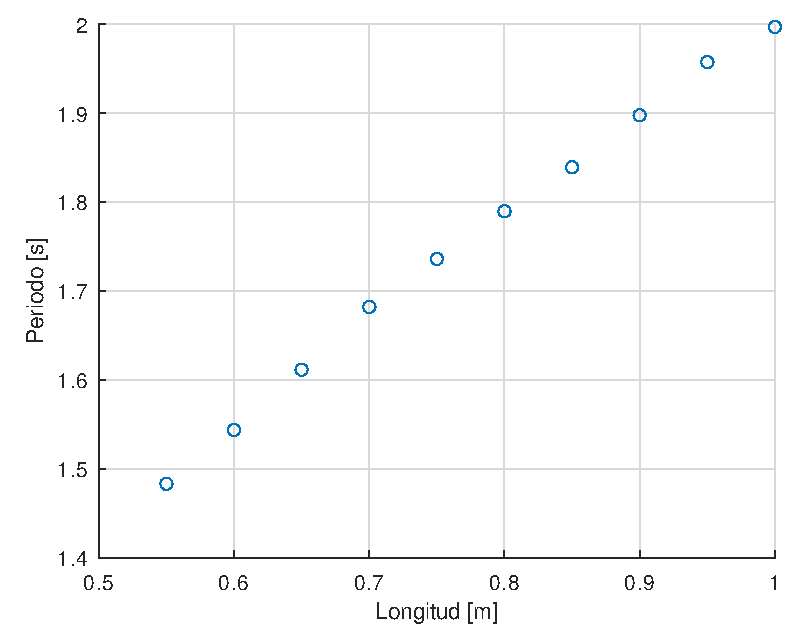
\includegraphics[width=0.75\textwidth]{resources/o1.1.eps}
\caption{Gráfica de longitud vs periodo.}
\label{figura3}
\source{Elaboración propia.}
\end{figure}

\section{Resultados}

A partir de los datos obtenidos se calculó el periodo de oscilación ($T$) para
los valores de longitud ($L$), con los que se generó la gráfica de la
\textbf{Figura \ref{figura3}}.

Posteriormente se linealizó la curva por medio de logaritmos, y se calculó la
recta de mejor ajuste por el método de los mínimos cuadrados, resultando los
siguientes valores:

\begin{equation*}
    A = (0.694 \pm 0.001) [u]; 0.23\%
\end{equation*}
\begin{equation*}
    B = (0.502 \pm 0.005) [u]; 0.98\%
\end{equation*}
\vspace{0.10cm}

Siendo su coeficiente de correlación ($r$):

\begin{equation*}
    r = 0.9996
\end{equation*}
\vspace{0.10cm}

Con los valores hallados, se calculan los valores originales de la curva,
resultando:

\begin{equation*}
    a = (2.002 \pm 0.003) [s/\sqrt{m}]; 0.16\%
\end{equation*}
\begin{equation*}
    b = (0.502 \pm 0.005) [u]; 0.98\%
\end{equation*}
\vspace{0.10cm}

Resultando el modelo de ajuste:

\begin{equation*}
    T = 2.002\,L^{0.502}
\end{equation*}
\vspace{0.10cm}

Por tanto la relación funcional entre $T$ y $L$, es:

\begin{center}
\begin{tabular}{|>{\centering}m{9.2cm}<{\centering}|}
\hline
\textbf{Resultado} 
\tabularnewline \hline
\\
$T \propto \sqrt{L}$ \tabularnewline
\\
\hline
\end{tabular}
\end{center}
\vspace{0.10cm}

Verificándose el comportamiento establecido por la
\textbf{Ecuación \ref{periodo}}.

Para el calculo de la gravedad ($g$) se utiliza la
\textbf{Ecuación \ref{gravedad}}, resultando:

\begin{center}
\begin{tabular}{|>{\centering}m{9.2cm}<{\centering}|}
\hline
\textbf{Resultado} 
\tabularnewline \hline
\\
$g = (9.85 \pm 0.03) [m/s^2]; 0.33\%$ \tabularnewline
\\
\hline
\end{tabular}
\end{center}
\vspace{0.10cm}

\section{Discusión}

Si se calculase la relación lineal entre la longitud ($L$) y el periodo ($T$)
directamente desde sus valores sin linealización previa, se obtienen los
siguientes valores de la recta:

\begin{equation*}
    A = (0.86 \pm 0.02) [s]; 2.08\%
\end{equation*}
\begin{equation*}
    B = (1.15 \pm 0.02) [s/\sqrt{m}]; 1.98\%
\end{equation*}
\vspace{0.10cm}

Siendo su coeficiente de correlación ($r$):

\begin{equation*}
    r = 0.9984
\end{equation*}
\vspace{0.10cm}

Considerando la correlación hallada, podría cometerse el error de presuponer una
relación lineal entre las variables. Esto se debe a que los datos tomados se
encuentran en una zona de la curva (que es una parábola) donde la curvatura es
muy alta ($[0.55, 1.00]$).

Se recomienda tener datos más dispersos para evitar una posible confusión de
este tipo.

\section{Conclusiones}

Se verificaron las ecuaciones planteadas en la introducción, así como la
ecuación de un oscilador armónico simple.

También se calculó el valor de la gravedad, siendo equivalente al valor
establecido en el simulador.

\begin{thebibliography}{99}

\bibitem{Young&Freedman} Young, Hugh D. y Freedman, Roger A. (2013).\\
Física Universitaria. Volumen 1.\\
13va Edición.\\
Capitulo 14.

\bibitem{GUIA} Departamento de Física - UMSS.\\
Laboratorio de Física Básica II.\\
Guía - Cartilla de laboratorio.\\
Gestión I/2020.

\bibitem{WIKI1} Péndulo simple \\
Extraído el 27 de Abril del 2021, de: \\
\url{https://es.wikipedia.org/wiki/P%C3%A9ndulo_simple}.

\end{thebibliography}

\newpage
\section*{Apéndice A: Cálculos adicionales}

\subsection{Linealización de la curva}

Conociendo $t_{1i}$, $t_{2i}$, se calculan los valores del promedio ($\bar{t}$),
y el periodo de oscilación ($T$) en el \textbf{Cuadro \ref{cuadro3}}.

\begin{table}[!h]
\begin{center}
\begin{tabular}{|c||>{\centering}m{2.0cm}<{\centering}
                  |>{\centering}m{2.0cm}<{\centering}
                  |>{\centering}m{2.0cm}<{\centering}|
                  |>{\centering}m{2.0cm}<{\centering}|}
\hline
$i$ & $t_{1i} [s]$ & $t_{2i} [s]$ & $\bar{t}_i [s]$ & $T_i [s]$
    \tabularnewline \hline \hline
 1 & $14.85$ & $14.81$ & $14.8300$ & $1.4830$ \tabularnewline \hline
 2 & $15.42$ & $15.45$ & $15.4350$ & $1.5435$ \tabularnewline \hline
 3 & $16.09$ & $16.14$ & $16.1150$ & $1.6115$ \tabularnewline \hline
 4 & $16.88$ & $16.76$ & $16.8200$ & $1.6820$ \tabularnewline \hline
 5 & $17.35$ & $17.37$ & $17.3600$ & $1.7360$ \tabularnewline \hline
 6 & $17.87$ & $17.92$ & $17.8950$ & $1.7895$ \tabularnewline \hline
 7 & $18.37$ & $18.41$ & $18.3900$ & $1.8390$ \tabularnewline \hline
 8 & $19.01$ & $18.94$ & $18.9750$ & $1.8975$ \tabularnewline \hline
 9 & $19.53$ & $19.62$ & $19.5750$ & $1.9575$ \tabularnewline \hline
10 & $20.02$ & $19.92$ & $19.9700$ & $1.9970$ \tabularnewline \hline
\end{tabular}
\caption{Calculo del periodo de oscilación.}
\label{cuadro3}
\source{Elaboración propia.}
\end{center}
\end{table}

En el \textbf{Cuadro \ref{cuadro4}}, se detallan los valores logaritmizados de
$T$ y $L$:

\begin{table}[!h]
\begin{center}
\begin{tabular}{|c||>{\centering}m{2.5cm}<{\centering}
                  |>{\centering}m{2.5cm}<{\centering}|}
\hline
$i$ & $ln(L_i)$ & $ln(T_i)$ \tabularnewline \hline \hline
 1 & -0.5978 & 0.3941 \tabularnewline \hline
 2 & -0.5108 & 0.4341 \tabularnewline \hline
 3 & -0.4308 & 0.4772 \tabularnewline \hline
 4 & -0.3567 & 0.5200 \tabularnewline \hline
 5 & -0.2877 & 0.5516 \tabularnewline \hline
 6 & -0.2231 & 0.5819 \tabularnewline \hline
 7 & -0.1625 & 0.6092 \tabularnewline \hline
 8 & -0.1054 & 0.6405 \tabularnewline \hline
 9 & -0.0513 & 0.6717 \tabularnewline \hline
10 &       0 & 0.6916 \tabularnewline \hline
\end{tabular}
\caption{Valores logaritmizados de $L$ y $T$.}
\label{cuadro4}
\source{Elaboración propia.}
\end{center}
\end{table}

\begin{figure}
\centering
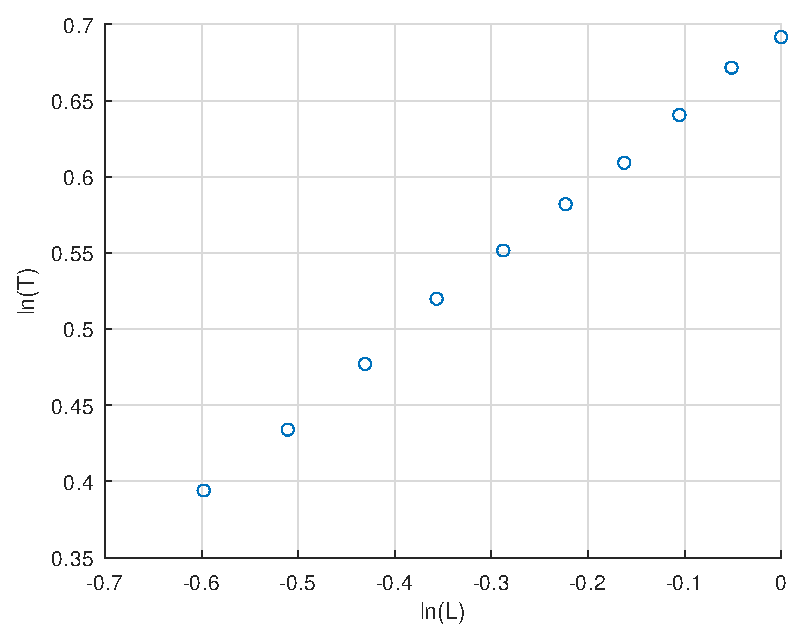
\includegraphics[width=0.75\textwidth]{resources/o1.2.eps}
\caption{Gráfica de $ln(L)$ vs. $ln(T)$.}
\label{figura4}
\source{Elaboración propia.}
\end{figure}

Los valores del \textbf{Cuadro \ref{cuadro4}}, pueden verse gráficamente en la
\textbf{Figura \ref{figura4}}.

\subsection{Método de mínimos cuadrados}

Se calculan los parámetros de la recta por el método de los mínimos cuadrados,
con la ayuda de los datos presentados en el \textbf{Cuadro \ref{cuadro5}}.

\begin{table}[!h]
\begin{center}
\begin{tabular}{|c||>{\centering}m{1.8cm}<{\centering}
                  |>{\centering}m{1.8cm}<{\centering}
                  |>{\centering}m{1.8cm}<{\centering}|
                  |>{\centering}m{1.8cm}<{\centering}
                  |>{\centering}m{1.8cm}<{\centering}
                  |>{\centering}m{2.1cm}<{\centering}|}
\hline
$i$ & $x^2_i$ & $y^2_i$ & $x_i y_i$ & $Y_i$ & $d_i$ & $d^2_i\,(\num{e-4})$
    \tabularnewline \hline \hline
 1 & 0.3574 & 0.1553 & -0.2356 & 0.3938 &  0.0002 & 0.0005
    \tabularnewline \hline
 2 & 0.2609 & 0.1884 & -0.2217 & 0.4375 & -0.0035 & 0.1222
    \tabularnewline \hline
 3 & 0.1856 & 0.2277 & -0.2056 & 0.4777 & -0.0006 & 0.0034
    \tabularnewline \hline
 4 & 0.1272 & 0.2704 & -0.1855 & 0.5150 &  0.0050 & 0.2516
    \tabularnewline \hline
 5 & 0.0828 & 0.3042 & -0.1587 & 0.5496 &  0.0020 & 0.0387
    \tabularnewline \hline
 6 & 0.0498 & 0.3386 & -0.1299 & 0.5820 & -0.0001 & 0.0001
    \tabularnewline \hline
 7 & 0.0264 & 0.3712 & -0.0990 & 0.6125 & -0.0033 & 0.1060
    \tabularnewline \hline
 8 & 0.0111 & 0.4103 & -0.0675 & 0.6412 & -0.0006 & 0.0042
    \tabularnewline \hline
 9 & 0.0026 & 0.4511 & -0.0345 & 0.6683 &  0.0033 & 0.1109
    \tabularnewline \hline
10 &      0 & 0.4784 &       0 & 0.6941 & -0.0025 & 0.0602
    \tabularnewline \hline
\end{tabular}
\caption{Valores para el método de mínimos cuadrados.}
\label{cuadro5}
\source{Elaboración propia.}
\end{center}
\end{table}

\begin{equation*}
    n = 10
\end{equation*}
\begin{equation*}
    \sum x_i = -2.7261
\end{equation*}
\begin{equation*}
    \sum y_i = 5.5719
\end{equation*}
\begin{equation*}
    \sum x^2_i = 1.1038
\end{equation*}
\begin{equation*}
    \sum y^2_i = 3.1956
\end{equation*}
\begin{equation*}
    \sum x_i y_i = -1.3378
\end{equation*}
\begin{equation*}
    \Delta_1 = n \sum x^2_i - \left( \sum x_i \right)^2 = 3.6067
\end{equation*}
\begin{equation*}
    \Delta_2 = n \sum y^2_i - \left( \sum y_i \right)^2 = 0.9104
\end{equation*}
\begin{equation*}
    A = \frac{\sum y_i \sum x^2_i - \sum x_i y_i \sum x_i}{\Delta_1} = 0.6941
\end{equation*}
\begin{equation*}
    B = \frac{n \sum x_i y_i - \sum x_i \sum y_i}{\Delta_1} = 0.5022
\end{equation*}
\begin{equation*}
    \sum d^2 = \num{6.9772e-5}
\end{equation*}
\begin{equation*}
    \sigma^2 = \frac{\sum d^2_i}{n-2} = \num{8.7215e-6}
\end{equation*}
\begin{equation*}
    \sigma_A = \sqrt{\frac{\sigma^2 \sum x^2_i}{\Delta_1}} = 0.0016
\end{equation*}
\begin{equation*}
    \sigma_B = \sqrt{\frac{\sigma^2 n}{\Delta_1}} = 0.0049
\end{equation*}
\vspace{0.10cm}

Parámetros de la recta obtenida:

\begin{equation*}
    A = (0.6941 \pm 0.0016) [u]; 0.2354 \%
\end{equation*}
\begin{equation*}
    B = (0.5022 \pm 0.0049) [u]; 0.9791 \%
\end{equation*}
\vspace{0.10cm}

Siendo el coeficiente de correlación:

\begin{equation*}
    R = \frac{n \sum x_i y_i - (\sum x_i)(\sum y_i)}{\sqrt{\Delta_1 \Delta_2}}
      = 0.9996
\end{equation*}
\vspace{0.10cm}

La ecuación de la recta resultante es:

\begin{equation*}
    y = 0.6941 + 0.5022\,x
\end{equation*}
\vspace{0.10cm}

A partir de los parámetros de recta $A$ y $B$, se calculan los parámetros $a$ y
$b$ de la curva original y sus errores por el método de propagación de errores:

\begin{equation*}
    a = e^{A} = e^{0.6941} = 2.0019
\end{equation*}
\begin{equation*}
    b = B = 0.5022
\end{equation*}
\begin{equation*}
    e_a = e^A e_A = e^{0.6941}\,(0.0016) = 0.0033
\end{equation*}
\begin{equation*}
    e_b = e_B = 0.0049
\end{equation*}
\vspace{0.10cm}

Obteniendo finalmente los valores de la curva:

\begin{equation*}
    a = (2.0019 \pm 0.0033) [s/\sqrt{m}]; 0.1634 \%
\end{equation*}
\begin{equation*}
    b = (0.5022 \pm 0.0049) [u]; 0.9791 \%
\end{equation*}
\vspace{0.10cm}

La ecuación de la curva resultante es:

\begin{equation*}
    T = a L^b = 2.0019\,d^{0.5022} = 2.0019\,\sqrt{d}
\end{equation*}
\vspace{0.10cm}

\subsection{Calculo de la gravedad}

Para el calculo de la gravedad, se utiliza la \textbf{Ecuación \ref{gravedad}}:

\begin{equation*}
    g = \frac{4 \pi^2}{a^2} = \frac{4(3.1415)^2}{(2.0019)^2} = 9.8508
\end{equation*}
\vspace{0.10cm}

Y el error de la medición es:

\begin{equation*}
    \frac{\partial g}{\partial a} = 4 \pi^2 (-2) a^{-3} = -\frac{8\pi^2}{a^3}
\end{equation*}
\begin{equation*}
    e_g = \frac{8 \pi^2}{a^3}\,e_a = 0.0322
\end{equation*}
\vspace{0.10cm}

Resultando:

\begin{equation*}
    g = (9.8508 \pm 0.0322) [m/s^2]; 0.3268\%
\end{equation*}
\vspace{0.10cm}

\newpage
\section*{Apéndice B: Cálculos realizados en \emph{Octave}}

A continuación se presenta los cálculos realizados en el programa \emph{Octave}
para la generación de las gráficas, la linealización de la curva, el calculo
de los mínimos cuadrados y el valor de la gravedad.

\begin{shaded}
\begin{alltt}
\footnotesize
\# Datos importados (i1.csv):
\input{resources/i1.csv}
\# Comandos ejecutados (o1.m):
\input{../../octave/graficar.m}
\input{../../octave/minimoscuadrados.m}
\input{resources/o1.m}
\# Salida del programa (o1.out):
\input{resources/o1.out}
\normalsize
\end{alltt}
\end{shaded}

\end{document}

